% Final presentation — Project 7
% Compile with XeLaTeX:
%   latexmk -xelatex -outdir=build main.tex
% or, without a local TeX Live install:
%   tectonic -X compile main.tex
%
% DRAFT SKELETON: numbers are the official v2 results (D-019); figures and
% the E / portfolio sections are placeholders to be filled in.

\documentclass[10pt, aspectratio=169]{beamer}

\usetheme{metropolis}
\metroset{progressbar=frametitle, numbering=fraction, block=fill, sectionpage=none}
\usepackage{appendixnumberbeamer}

\usepackage{booktabs}
\usepackage{amsmath, amssymb, mathtools, bm}
\usepackage{xspace}
\usepackage{tikz}
\usetikzlibrary{arrows.meta, positioning, shapes.geometric, calc, fit, backgrounds}
\usepackage{pgfplots}
\pgfplotsset{compat=1.18}
\usepackage{array}

% ---- Bibliography (author-year) ----
\usepackage[style=authoryear, maxcitenames=2, maxbibnames=10, giveninits=true,
            uniquename=false, backend=bibtex, doi=false, isbn=false, url=false, eprint=true]{biblatex}
\addbibresource{refs.bib}
\renewcommand*{\bibfont}{\scriptsize}
\renewcommand*{\multicitedelim}{\addcomma\space}
\renewcommand*{\multinamedelim}{\addcomma\space}
\renewcommand*{\finalnamedelim}{\addspace\bibstring{and}\space}
\renewcommand*{\finentrypunct}{\addperiod}
\DeclareFieldFormat[article,misc]{title}{#1}
\DeclareFieldFormat{journaltitle}{\mkbibemph{#1}}
\renewbibmacro{in:}{}
\DeclareFieldFormat[article]{volume}{#1}
\DeclareFieldFormat[article]{number}{\mkbibparens{#1}}
\DeclareFieldFormat[article]{pages}{#1}
\DeclareFieldFormat{eprint:arxiv}{arXiv\addcolon\space #1}
\renewbibmacro*{volume+number+eid}{%
  \printfield{volume}%
  \printfield{number}%
  \setunit{\addcomma\space}%
  \printfield{eid}}
\setbeamertemplate{bibliography item}{}
\setbeamerfont{bibliography entry title}{series=\mdseries}
\setbeamertemplate{frametitle continuation}{}
\setbeamercolor{bibliography entry author}{fg=black!85}
\setbeamercolor{bibliography entry title}{fg=black!85}
\setbeamercolor{bibliography entry location}{fg=black!70}
\setbeamercolor{bibliography entry note}{fg=black!70}

% ---- Palette: restrained, journal-like (same as the mid-term deck) ----
\definecolor{navy}{HTML}{1F3A5F}
\definecolor{slate}{HTML}{4A5A6A}
\definecolor{accent}{HTML}{B5462E}
\definecolor{lightbg}{HTML}{F2F4F7}
\definecolor{green2}{HTML}{3F7F5F}
\setbeamercolor{frametitle}{bg=navy, fg=white}
\setbeamercolor{progress bar}{fg=accent, bg=lightbg}
\setbeamercolor{title separator}{fg=accent}
\setbeamercolor{normal text}{fg=black!85}
\setbeamercolor{alerted text}{fg=accent}
\setbeamercolor{block title}{bg=navy!12, fg=navy}
\setbeamercolor{block body}{bg=lightbg}
\setbeamercolor{background canvas}{bg=white}
\setbeamertemplate{itemize item}{\color{navy}$\bullet$}
\setbeamertemplate{itemize subitem}{\color{slate}\scriptsize$\blacktriangleright$}

% ---- Tighter lists ----
\let\olditemize\itemize
\renewcommand{\itemize}{\olditemize\setlength{\itemsep}{0.35ex}\setlength{\parskip}{0pt}}
\usepackage{array}
\newcolumntype{L}[1]{>{\raggedright\arraybackslash}p{#1}}

% ---- Numbered captions ----
\setbeamertemplate{caption}[numbered]
\setbeamertemplate{caption label separator}{.\ }
\setbeamerfont{caption}{size=\scriptsize}
\setbeamerfont{caption name}{size=\scriptsize, series=\bfseries}
\setbeamercolor{caption name}{fg=navy}

% ---- Helpers ----
\newcommand{\E}{\mathbb{E}}
\newcommand{\where}{{\footnotesize\color{slate}where}}
\newcommand{\paperref}[1]{{\scriptsize\color{slate}\AtNextCitekey{\defcounter{maxnames}{99}}\fullcite{#1}\par}\vspace{0.4ex}}
\newcommand{\smallnote}[1]{{\footnotesize\color{slate}#1}}
\newcommand{\hl}[1]{\textcolor{accent}{#1}}
\newcommand{\key}[1]{\textcolor{accent}{\textbf{#1}}}
\newcommand{\takeaway}[1]{%
  \vspace{0.6ex}%
  \begin{beamercolorbox}[rounded=true,sep=0.55ex,wd=\linewidth]{block body}%
    {\scriptsize\color{navy}\textbf{Takeaway.}~#1}%
  \end{beamercolorbox}}
\newcommand{\figph}[2][4.2cm]{%
  \begin{tikzpicture}
    \node[draw=slate!40, dashed, fill=lightbg, rounded corners=2pt,
          text width=0.84\linewidth, minimum height=#1, align=center,
          font=\scriptsize, text=slate, inner sep=4pt] {#2};
  \end{tikzpicture}}
\tikzset{
  box/.style={draw=navy, fill=navy!6, rounded corners=2pt, align=center,
              font=\scriptsize, minimum height=0.8cm, text width=2.0cm, line width=0.5pt},
  boxacc/.style={box, draw=accent, fill=accent!7},
  arr/.style={-{Stealth[length=2mm]}, line width=0.6pt, color=slate},
}

\newcommand{\deckfooter}{%
  \tiny\color{slate}MTH 9897 \textperiodcentered\ Project 7 \textperiodcentered\ Commodity calendar spreads}
\setbeamertemplate{frame footer}{\deckfooter}

\title{Systematic Trading}
\subtitle{Project 7: Commodity Futures Calendar Spreads}
\author{Jiaheng Han \& Tian Tian}
\institute{Baruch College, MFE Program}
\date{October 2026}

\begin{document}

% =====================================================================
\begin{frame}[plain]
  \titlepage
\end{frame}

% =====================================================================
\section{Setup}

\begin{frame}{Project 7: what we study}
\begin{columns}[T, onlytextwidth]
\begin{column}{0.55\textwidth}
\footnotesize
\begin{itemize}
  \item A futures curve prices the \key{same commodity} at different delivery months
  \item A calendar spread trades two points on that curve
  \[
    C_t = F(t,T_1) - F(t,T_2), \qquad T_1 < T_2
  \]
  \item Long the spread: long the near contract, short the far one; P\&L is
        $q\,M\,\Delta C_{t+h}$
  \item The flat price largely cancels; what remains is the \key{shape of the curve},
        roll and convergence
  \item Research question: does term-structure information predict the spread
        change, \key{net of rolls and costs}?
\end{itemize}
\end{column}
\begin{column}{0.42\textwidth}
\begin{figure}
\centering
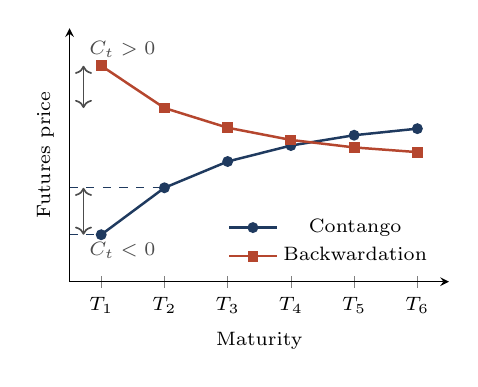
\begin{tikzpicture}
\begin{axis}[
  width=6.4cm, height=4.8cm,
  xlabel={\scriptsize Maturity}, ylabel={\scriptsize Futures price},
  xmin=0.5, xmax=6.5, ymin=57, ymax=84, clip=false,
  xtick={1,2,3,4,5,6}, xticklabels={$T_1$,$T_2$,$T_3$,$T_4$,$T_5$,$T_6$},
  ytick=\empty, tick label style={font=\scriptsize},
  axis lines=left, legend columns=1,
  legend style={font=\scriptsize, draw=none, at={(0.98,0.02)}, anchor=south east},
  every axis plot/.append style={line width=0.9pt, mark size=1.5pt}]
\addplot[color=navy, mark=*] coordinates {(1,62) (2,67) (3,69.8) (4,71.5) (5,72.6) (6,73.3)};
\addlegendentry{Contango}
\addplot[color=accent, mark=square*] coordinates {(1,80) (2,75.5) (3,73.4) (4,72.1) (5,71.3) (6,70.8)};
\addlegendentry{Backwardation}
\draw[dashed, color=navy, line width=0.5pt] (axis cs:0.5,62) -- (axis cs:1,62);
\draw[dashed, color=navy, line width=0.5pt] (axis cs:0.5,67) -- (axis cs:2,67);
\draw[<->, color=black!70, line width=0.6pt] (axis cs:0.72,62) -- (axis cs:0.72,67);
\node[font=\scriptsize, color=black!70, anchor=north west, inner sep=1pt] at (axis cs:0.76,61.5) {$C_t<0$};
\draw[<->, color=black!70, line width=0.6pt] (axis cs:0.72,75.5) -- (axis cs:0.72,80);
\node[font=\scriptsize, color=black!70, anchor=south west, inner sep=1pt] at (axis cs:0.76,80.5) {$C_t>0$};
\end{axis}
\end{tikzpicture}
\caption{Stylized futures curves. The arrow is the calendar spread.}
\end{figure}
\end{column}
\end{columns}
\end{frame}

% =====================================================================
\begin{frame}{Data: Bloomberg bulk export, 1986--2026}
\begin{columns}[T, onlytextwidth]
\begin{column}{0.55\textwidth}
\footnotesize
\begin{itemize}
  \item Source: \key{Bloomberg bulk export} of generic futures ranks
  \item 24 commodities $\times$ four nearby ranks (M1--M4), daily
  \item Sample: \key{1986-01-01 to 2026-10-13}, 10{,}640 trading days
  \item Four fields: settlement, volume, open interest, current generic ticker
  \item M1--M4 are \key{slots, not contracts}; the ticker identifies the real contract
  \item Known edges: XB starts in 2005, LB ends in 2023; CL on 2020-04-20 is
        $-37.63$ and is kept
\end{itemize}
\end{column}
\begin{column}{0.42\textwidth}
\centering
{\scriptsize
\setlength{\tabcolsep}{3pt}
\begin{tabular}{@{}l l@{}}
\toprule
Sector & Roots \\
\midrule
Energy (5)      & CL, CO, HO, NG, XB \\
Grains (4)      & C, O, RR, W \\
Oilseeds (3)    & BO, S, SM \\
Softs (4)       & CC, JO, KC, SB \\
Industrials (2) & CT, LB \\
Livestock (3)   & FC, LC, LH \\
Metals (3)      & GC, HG, SI \\
\midrule
Total           & 24 \\
\bottomrule
\end{tabular}
\par}
\vspace{1ex}
{\scriptsize\color{slate}CME, CBOT, NYMEX, COMEX and ICE contracts.}
\end{column}
\end{columns}
\end{frame}

% =====================================================================
\begin{frame}{From slots to contracts: the panel}
\begin{columns}[T, onlytextwidth]
\begin{column}{0.55\textwidth}
\footnotesize
\begin{itemize}
  \item Rank panel $\rightarrow$ contract panel: each row is a date $\times$
        \key{real contract}; 6{,}735 contracts, 950{,}626 contract-days
  \item Returns are computed on contract codes; on a roll the new M1 inherits
        the old M2's previous price
  \item \key{Never difference generic prices across a roll}: that jump is a
        spread, not a return
  \item Eligibility: no delivery month; exit at least 5 trading days before;
        days to last trading $> D=10$ \smallnote{(D=5/20 are robustness only)}
\end{itemize}
\end{column}
\begin{column}{0.42\textwidth}
\centering
{\scriptsize
\setlength{\tabcolsep}{3pt}
\begin{tabular}{@{}l r@{}}
\toprule
Panel & Rows \\
\midrule
Rank                & 1{,}013{,}664 \\
Contract            & 950{,}626 \\
Returns             & 1{,}013{,}664 \\
Main pairs          & 236{,}186 \\
Spread              & 236{,}186 \\
Universe            & 236{,}186 \\
Adjacent pairs      & 610{,}801 \\
\bottomrule
\end{tabular}
\par}
\vspace{1ex}
{\scriptsize\color{slate}All panels are rebuilt from the raw CSV.}
\end{column}
\end{columns}
\end{frame}

% =====================================================================
\begin{frame}{One engine for all five ideas}
\footnotesize
\begin{itemize}
  \item v2 is holdings-based: \texttt{marks $\rightarrow$ sizing $\rightarrow$
        simulate $\rightarrow$ report}
  \item Signal at $t$ close; \key{fill at $t+1$ close}; existing positions are
        marked before orders
  \item All-in cost: \key{half-spread + exchange fee + square-root impact}
  \item Eligibility: at least 5 sessions before the delivery month; more than
        5 days to last trading; thinner-leg lagged average daily volume at
        least 100 contracts
  \item USD 10m book, equal notional; weekly, monthly or daily rebalance by idea
  \item Full 1986--2026; train 1986--2015; \key{test 2016--2026 read once, no tuning}
  \item Report gross and all-in net: annualized return, Sharpe, turnover, drawdown
\end{itemize}
\begin{center}
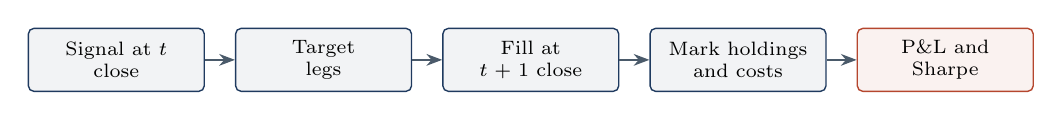
\begin{tikzpicture}[node distance=0.38cm]
\node[box] (sig) {Signal at $t$\\close};
\node[box, right=of sig] (tgt) {Target\\legs};
\node[box, right=of tgt] (fill) {Fill at\\$t+1$ close};
\node[box, right=of fill] (mark) {Mark holdings\\and costs};
\node[boxacc, right=of mark] (pnl) {P\&L and\\Sharpe};
\draw[arr] (sig) -- (tgt);
\draw[arr] (tgt) -- (fill);
\draw[arr] (fill) -- (mark);
\draw[arr] (mark) -- (pnl);
\end{tikzpicture}
\end{center}
\end{frame}

% =====================================================================
\begin{frame}{Roadmap: five ideas, one pipeline}
\centering
{\scriptsize
\setlength{\tabcolsep}{3pt}
\begin{tabular}{@{}l L{3.05cm} L{3.45cm} L{2.75cm}@{}}
\toprule
\textbf{Idea} & \textbf{Design} & \textbf{Reference} & \textbf{Verdict} \\
\midrule
\textbf{A} & Spread convergence
          & \textcite{kanamura2010profit}
          & candidate (gross) \\
\textbf{B} & Curve relative-value convergence
          & ---
          & candidate (gross) \\
\textbf{C} & Spread mean reversion
          & \textcite{lubnau2015trading} & weak gross \\
\textbf{D} & Curve momentum
          & \textcite{paschke2020curve} & weak / negative \\
\textbf{E} & Nelson--Siegel dynamics
          & \textcite{bianchi2023exploiting} & teammate \\
\bottomrule
\end{tabular}
\par}
\vspace{1.5ex}
{\footnotesize\color{slate}Same data, same eligibility, same engine, same
all-in costs. \key{Only the signal changes.}\\[2pt]
A/B are convergence designs; C/D/E are paper-based.}
\end{frame}

% =====================================================================
\section{A: Spread convergence}

\begin{frame}{A \textperiodcentered\ Spread convergence: the idea}
\begin{columns}[T, onlytextwidth]
\begin{column}{0.55\textwidth}
\footnotesize
\begin{itemize}
  \item A calendar spread should \key{converge}: the near and far contracts
        cannot stay apart forever
  \item Spread: $C_t = F_{\text{near}} - F_{\text{far}}$; convergence means
        $C_t \rightarrow 0$
  \item If $C_t < 0$ (contango), the spread is cheap: \key{long the spread}
  \item If $C_t > 0$ (backwardation), the spread is rich: \key{short the spread}
  \item Trade the main pair: long the near contract and short the far one,
        or the reverse
\end{itemize}
\end{column}
\begin{column}{0.42\textwidth}
\centering
{\scriptsize
\setlength{\tabcolsep}{5pt}
\begin{tabular}{@{}l l@{}}
\toprule
State & Position \\
\midrule
Contango ($C_t<0$)      & long spread \\
Backwardation ($C_t>0$) & short spread \\
\bottomrule
\end{tabular}
\par}
\vspace{1.5ex}
\begin{block}{Related paper}
{\scriptsize \textcite{kanamura2010profit} model spread trading as a
mean-reverting process with first-hitting times. In energy futures, profits
depend on spread volatility and the speed of mean reversion.}
\end{block}
\end{column}
\end{columns}
\end{frame}

% =====================================================================
\begin{frame}{A \textperiodcentered\ Spread convergence: backtest and robustness}
\centering
{\scriptsize
\setlength{\tabcolsep}{5pt}
\begin{tabular}{@{}l r r r r@{}}
\toprule
Period & Gross (\%/yr) & Sharpe & NW $t$ & 80\% MDE Sharpe \\
\midrule
Full 1986--2026 & $+0.63$ & $0.63$ & $4.29$ & $0.43$ \\
Train 1986--2015 & $+0.69$ & $0.67$ & $4.06$ & $0.51$ \\
Test 2016--2026 & $+0.46$ & $0.51$ & $1.58$ & $0.84$ \\
\bottomrule
\end{tabular}
\par}
\vspace{0.5ex}
{\scriptsize\color{slate}Gross-only, 0.5$\times$ equal notional; transaction costs are deferred to the portfolio.}
\vspace{1ex}
\begin{columns}[T, onlytextwidth]
\begin{column}{0.54\textwidth}
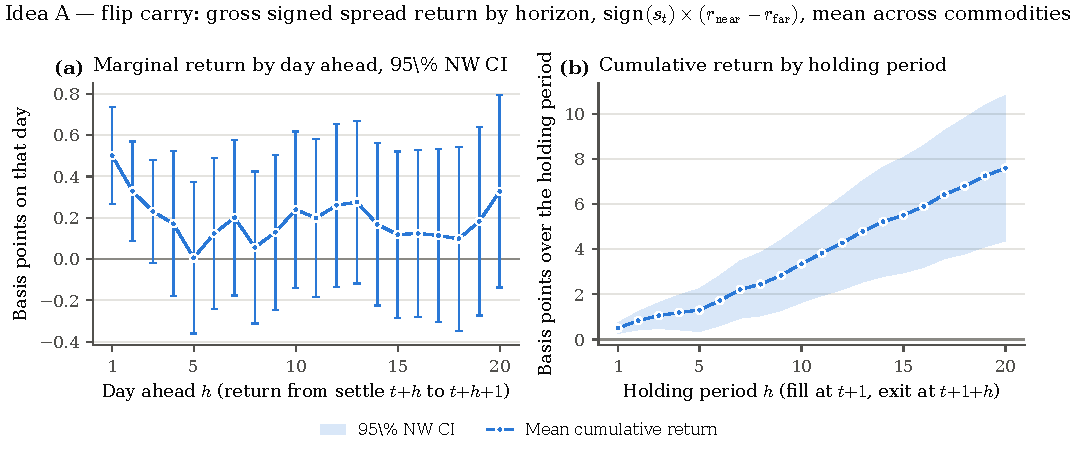
\includegraphics[width=\linewidth]{figures/a_flip_horizon_decay.pdf}
\par
{\scriptsize\color{slate}1$\times$ spread return: marginal (left) and cumulative (right).}
\end{column}
\begin{column}{0.43\textwidth}
\footnotesize
\begin{itemize}
  \item Timing: $t+1$ fill $+0.63\%$/yr vs same-settle $+0.71\%$;
        the edge survives the one-day lag
  \item 5-day IC $0.048$ / $0.045$ / $0.071$; roots with $p<0.05$:
        11/24, 10/24, 8/24
  \item Test $+0.46\%$, Sharpe $0.51$ vs MDE $0.84$:
        \key{suggestive, not confirmed}
\end{itemize}
\end{column}
\end{columns}
\end{frame}

% =====================================================================
\begin{frame}{A \textperiodcentered\ Spread convergence: position book and gross P\&L}
\begin{columns}[T, onlytextwidth]
\begin{column}{0.54\textwidth}
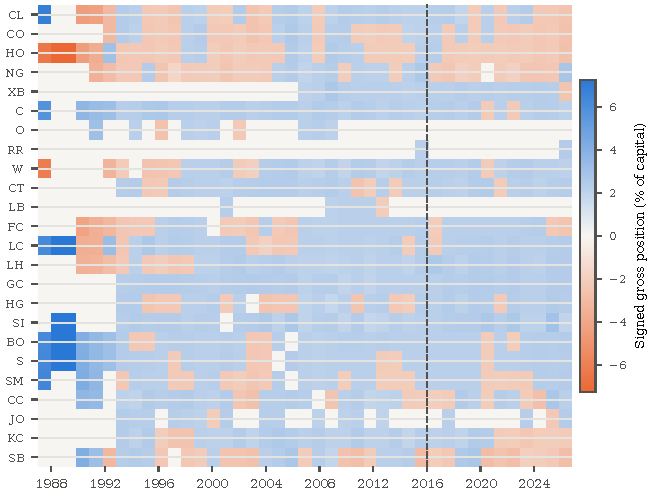
\includegraphics[width=0.92\linewidth]{figures/a_convergence_positions.pdf}
{\scriptsize\color{slate}Year-end position; blue = long near, orange = short.}
\end{column}
\begin{column}{0.43\textwidth}
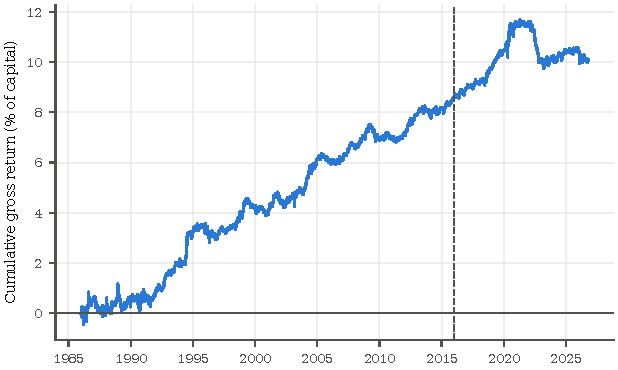
\includegraphics[width=0.92\linewidth]{figures/a_convergence_pnl.pdf}
{\scriptsize\color{slate}Gross P\&L, v2 simulator, 0.5$\times$ target.}
\vspace{0.5ex}
\begin{itemize}
  \item Book: long contango, short backwardation; heavy in the early 1990s
  \item Gross P\&L trends up; the table's $+0.63\%$ is the 5-day information
        test
\end{itemize}
\end{column}
\end{columns}
\end{frame}

% =====================================================================
\section{B: Curve relative value convergence}

\begin{frame}{B \textperiodcentered\ Curve relative value convergence: the idea}
\begin{columns}[T, onlytextwidth]
\begin{column}{0.55\textwidth}
\footnotesize
\begin{itemize}
  \item Within one curve, adjacent spreads should \key{converge in relative value}
  \item At each date and root, compute annualized carry for
        M1--M2, M2--M3, M3--M4
  \item \key{Long the lowest-carry adjacent spread}, \key{short the highest}
  \item Four legs; shared legs net out, so the book is a relative-value bet
        on one curve
  \item The extreme carry points should not stay extreme forever
\end{itemize}
\end{column}
\begin{column}{0.42\textwidth}
\centering
{\scriptsize
\setlength{\tabcolsep}{4pt}
\begin{tabular}{@{}l c c@{}}
\toprule
Adjacent spread & Carry & Position \\
\midrule
M1--M2 & low  & long \\
M2--M3 & mid  & --- \\
M3--M4 & high & short \\
\bottomrule
\end{tabular}
\par}
\vspace{0.5ex}
{\scriptsize\color{slate}Illustration only, not data.}
\end{column}
\end{columns}
\end{frame}

% =====================================================================
\begin{frame}{B \textperiodcentered\ Curve relative value convergence: backtest and robustness}
\centering
{\scriptsize
\setlength{\tabcolsep}{5pt}
\begin{tabular}{@{}l r r l@{}}
\toprule
Design & Gross (\%/yr) & Sharpe & Note \\
\midrule
Convergence & $+0.50$ & $1.06$ & NW $t=7.14$; turnover $31.4\times$ \\
Static front/back & $+0.11$ & $0.21$ & no relative-value ranking \\
\bottomrule
\end{tabular}
\par}
\vspace{0.5ex}
{\scriptsize\color{slate}Full sample 1986--2026; gross only. Fixed specification; 2016--2026 is a stability slice, not OOS.}
\vspace{1ex}
\begin{columns}[T, onlytextwidth]
\begin{column}{0.48\textwidth}
\footnotesize
\begin{itemize}
  \item 37/41 years positive; 22/24 roots positive; random-ranking placebo $p<0.001$
  \item Signal level: 6-day $+3.98$ bp ($t=9.6$); 21-day $+12.4$ bp ($t=8.6$)
  \item \$1m whole lots: gross $+0.28\%$/yr, Sharpe $0.29$; sizing matters
\end{itemize}
\end{column}
\begin{column}{0.48\textwidth}
\footnotesize
\begin{itemize}
  \item Half-spread alone is \key{84 bps/yr} vs 50 bps gross;
        all-in net about $-2.0\%$/yr
  \item Top roots include thin contracts (JO, LB, RR): capacity needs work
  \item \key{Not standalone}; a portfolio candidate
\end{itemize}
\end{column}
\end{columns}
\end{frame}

% =====================================================================
\begin{frame}{B \textperiodcentered\ Curve relative value convergence: position book and gross P\&L}
\begin{columns}[T, onlytextwidth]
\begin{column}{0.54\textwidth}
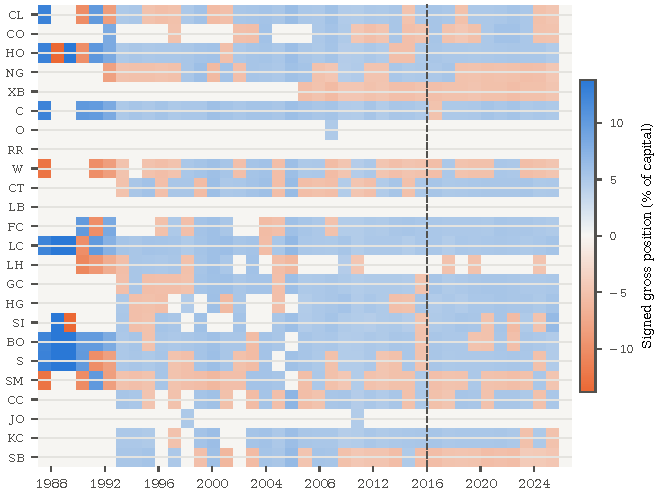
\includegraphics[width=\linewidth]{figures/b_convergence_positions.pdf}
{\scriptsize\color{slate}Year-end position; blue = long near, orange = short.}
\end{column}
\begin{column}{0.43\textwidth}
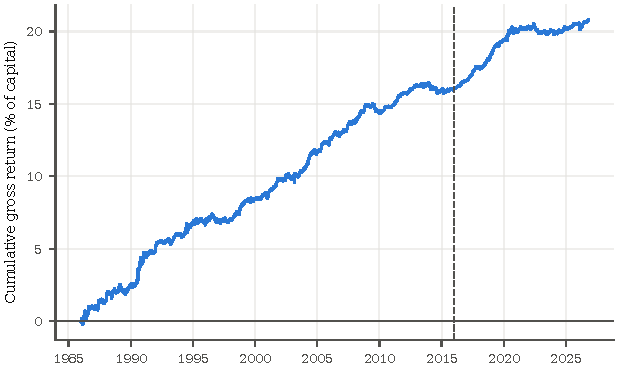
\includegraphics[width=\linewidth]{figures/b_convergence_pnl.pdf}
{\scriptsize\color{slate}Gross P\&L, v2 simulator.}
\vspace{0.5ex}
\begin{itemize}
  \item The four-leg book rotates across roots; positions are diversified
  \item Gross P\&L $+0.50\%$/yr; half-spread alone is 84 bps, so costs still
        consume it
\end{itemize}
\end{column}
\end{columns}
\end{frame}

% =====================================================================
\section{C: Spread mean reversion}

\begin{frame}{C \textperiodcentered\ Spread mean reversion: the idea}
\paperref{lubnau2015trading}
\begin{columns}[T, onlytextwidth]
\begin{column}{0.56\textwidth}
\footnotesize
\begin{itemize}
  \item The trade is the \key{residual}, not the price level: hedge the near
        contract $A$ with the far contract $B$,
        $p_{H,t} = p_{A,t} - \beta_t\,p_{B,t}$
  \item Standardize the residual:
        $z_t = (p_{H,t} - \mathrm{MA}_{20,t})/\sigma_{20,t}$
  \item \key{Long $z_t<-2$, short $z_t>2$, exit at $z_t=0$}
  \item Three hedge ratios: \key{1:1 dollar} (headline),
        \key{60-day rolling OLS}, \key{Kalman DLM}
  \item 24 commodities, 1986--2026; main pair; weekly rebalance; $t+1$ fill;
        gross-only
\end{itemize}
\end{column}
\begin{column}{0.41\textwidth}
\centering
{\scriptsize
\setlength{\tabcolsep}{4pt}
\begin{tabular}{@{}L{1.95cm} L{3.35cm}@{}}
\toprule
Paper & This project \\
\midrule
Energy only & 24 commodities \\
1992--2013 & 1986--2026 \\
Front vs 2--5 & Main pair \\
Sharpe above 2 & gross Sharpe 0.38 \\
\bottomrule
\end{tabular}
\par}
\vspace{1.2ex}
\begin{block}{Why three hedge ratios}
{\scriptsize The hedge ratio is the key degree of freedom, and with four
contracts it is unstable.}
\end{block}
\end{column}
\end{columns}
\end{frame}

% =====================================================================
\begin{frame}{C \textperiodcentered\ Spread mean reversion: gross backtest and robustness}
\centering
{\scriptsize
\setlength{\tabcolsep}{5pt}
\begin{tabular}{@{}l r r r r@{}}
\toprule
Variant & Gross (\%/yr) & Gross Sharpe & NW $t$ & Test gross \\
\midrule
C1 1:1 dollar   & $+0.61$ & $0.38$ & $2.62$ & $+0.16$ \\
C2 rolling OLS  & $+0.12$ & $0.11$ & $0.69$ & $-0.01$ \\
C3 Kalman DLM   & $+0.61$ & $0.25$ & $1.62$ & $+0.98$ \\
\bottomrule
\end{tabular}
\par}
\vspace{0.3ex}

{\scriptsize
\setlength{\tabcolsep}{4pt}
\begin{tabular}{@{}L{3.30cm} L{10.35cm}@{}}
\toprule
Robustness check & Result \\
\midrule
Three hedge ratios & C1/C2/C3 gross $+0.61/+0.12/+0.61$; gross Sharpe $0.38/0.11/0.25$ \\
Train $\rightarrow$ test gross & C1 $+0.78 \rightarrow +0.16$; C2 $+0.17 \rightarrow -0.01$; C3 $+0.48 \rightarrow +0.98$ \\
Daily validation SR & C1 $0.240$, C2 $0.265$, C3 $-0.332$; alpha gate $0.4$ failed \\
Execution lag / placebo & same-settle $0.419 \rightarrow$ tradable $0.064$; placebo $p=0.656$ \\
Breadth / jackknife & 15/24 validation roots positive; drop LH $0.448$; drop NG/CT/CC $0.12$ \\
IC / OOS $R^2$ & 1/5/10/20d IC $0.010/0.003/-0.001/0.021$; OOS $R^2<0$ \\
\bottomrule
\end{tabular}
\par}
\vspace{0.2ex}
{\scriptsize\color{slate}Gross-only; costs are deferred to the portfolio.
Weekly = official D-019; daily audit = validation only;
test rows are descriptive/post-hoc, not OOS.}\par
\vspace{0.3ex}
{\scriptsize\color{navy}\textbf{Why the paper differs.} Sharpe $>2$ is an
energy-subset result from a large grid, not a broad strategy; likely
post-selection. Our gross Sharpe is $0.38$; on the paper sample,
CL $-0.26$, NG $+0.31$.}
\end{frame}

% =====================================================================
\begin{frame}{C \textperiodcentered\ Spread mean reversion: position book and gross P\&L}
\begin{columns}[T, onlytextwidth]
\begin{column}{0.50\textwidth}
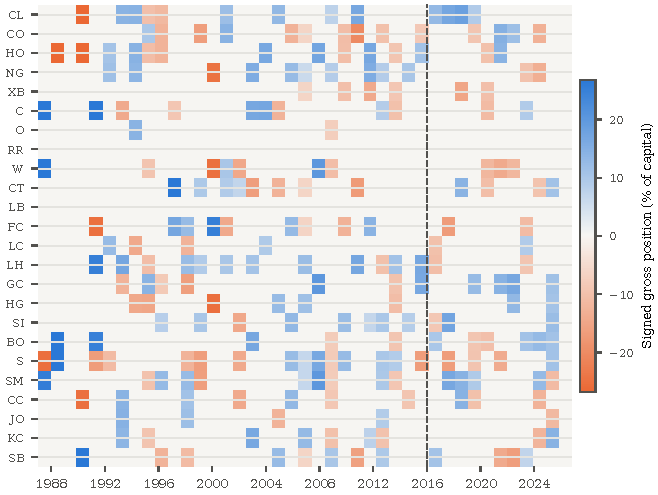
\includegraphics[width=\linewidth]{figures/c_mean_reversion_positions.pdf}
{\scriptsize\color{slate}Year-end position; blue = long near, orange = short.}
\end{column}
\begin{column}{0.47\textwidth}
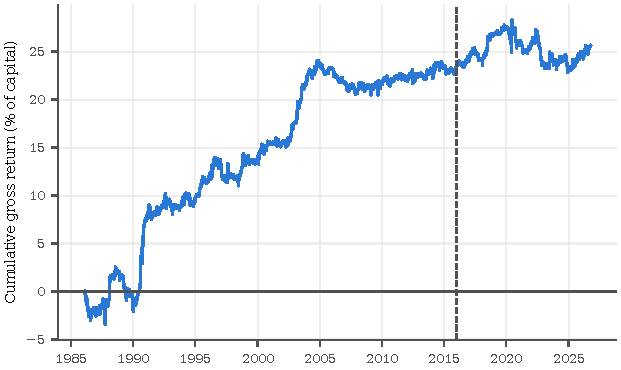
\includegraphics[width=\linewidth]{figures/c_mean_reversion_pnl.pdf}\par
{\scriptsize\color{slate}Gross P\&L, \$10m capital; dashed line = 2016.}
\vspace{0.3ex}
\footnotesize
\begin{itemize}
  \item Book rotates across all 24 roots; no persistent directional tilt
  \item Gross $+0.61\%$/yr full sample; $+0.16\%$/yr test
  \item Gross P\&L drifts up but the slope is small and unstable
\end{itemize}
\end{column}
\end{columns}
\end{frame}

% =====================================================================
\section{D: Curve momentum}

\begin{frame}{D \textperiodcentered\ Curve momentum: the trade idea}
\begin{columns}[T, onlytextwidth]
\begin{column}{0.57\textwidth}
\footnotesize
\begin{itemize}
  \item Within one commodity's curve, compare the two nearest tradable
        contracts (near = earlier expiry, far = later expiry); this is a
        \key{relative} trade, not a long or short commodity bet
  \item For each leg, compound its roll-adjusted daily rank return over the
        past \key{12 months}:
        $m_{i,t}=\prod_{s\in[t-12m,\,t]}(1+r_{i,s})-1$
  \item Signal: \key{$score_t=m_{near,t}-m_{far,t}$}
  \item If $score_t>0$, \key{long the near leg, short the far leg};
        if $score_t<0$, reverse. Hold \key{one month}
  \item Month-end close signal, \key{$t+1$ close fill}; the target is held
        until the next month-end; monthly rebalance
  \item Economic story: relative curve momentum persists over the next month;
        the contract that has outperformed stays stronger
\end{itemize}
\vspace{0.2ex}
{\scriptsize\color{slate}Reference: \textcite{paschke2020curve}.}
\end{column}
\begin{column}{0.40\textwidth}
\centering
{\scriptsize
\setlength{\tabcolsep}{2pt}
\begin{tabular}{@{}L{2.35cm} L{3.15cm}@{}}
\toprule
Parameter & Choice \\
\midrule
Universe & 24 roots, 1986--2026 \\
Legs & $N=2$ main pair \\
Formation & 12 months \\
Holding & 1 month \\
Signal & $m_{near}-m_{far}$ \\
Position & $\operatorname{sign}(score)$, $\pm1$ per leg \\
Sizing & equal notional \\
Delivery rule & no delivery month; $k=5$ \\
Expiry buffer & $d=5$ days to last trading \\
Liquidity & thinner-leg ADV $\ge100$ \\
Execution & month-end $\rightarrow$ $t+1$ close \\
Costs & gross-only \\
\bottomrule
\end{tabular}
\par}
\vspace{0.8ex}
{\scriptsize\color{slate}Official v2 all-in net: $-1.42\%$/yr;
turnover $22\times$/yr.}
\end{column}
\end{columns}
\end{frame}

% =====================================================================
\begin{frame}{D \textperiodcentered\ Curve momentum: backtest and robustness}
\centering
{\scriptsize
\setlength{\tabcolsep}{5pt}
\begin{tabular}{@{}l r r r r@{}}
\toprule
Period & Gross (\%/yr) & Sharpe & NW $t$ & 80\% MDE Sharpe \\
\midrule
Full 1986--2026 & $+0.22$ & $0.25$ & $1.77$ & $0.43$ \\
Train 1986--2015 & $+0.37$ & $0.41$ & $2.60$ & $0.51$ \\
Test 2016--2026 & $-0.21$ & $-0.26$ & $-0.83$ & $0.84$ \\
\bottomrule
\end{tabular}
\par}
\vspace{0.2ex}
{\scriptsize\color{slate}Gross-only, \$10m capital, equal notional. Official v2
all-in net: $-1.42\%$/yr, turnover $22\times$/yr. Test is a post-hoc
stability slice, not a new OOS selection.}
\vspace{0.8ex}

{\scriptsize
\setlength{\tabcolsep}{3pt}
\begin{tabular}{@{}L{2.30cm} L{7.55cm} L{3.75cm}@{}}
\toprule
Check & Data & Conclusion \\
\midrule
Core IC & 1m IC $0.049$ (NW $t$ 3.48); $79\%$ roots $+$; hit $52.5\%$; FDR $2/24$ & small, concentrated \\
Horizon & IC $0.049/0.140/0.173/0.190$ at 1/3/6/12m & slow; most beyond 1m \\
Independence & $\Delta$adj $R^2$ $+0.0069$ (CI includes 0); residual IC $+0.016$; static $11.1$ vs timing $11.2$ bp/m & no incremental value \\
Stability & 1986--99 IC $0.013$; high-vol IC $-0.007$; rolling 36m positive $39\%$ & unstable over time \\
Placebo & block shuffle $p<0.001$; lag-1m IC $0.016$; future-score lead $0.028$ & not noise; persistent/static \\
\bottomrule
\end{tabular}
\par}
\end{frame}

% =====================================================================
\begin{frame}{D \textperiodcentered\ Curve momentum: position book and gross P\&L}
\begin{columns}[T, onlytextwidth]
\begin{column}{0.50\textwidth}
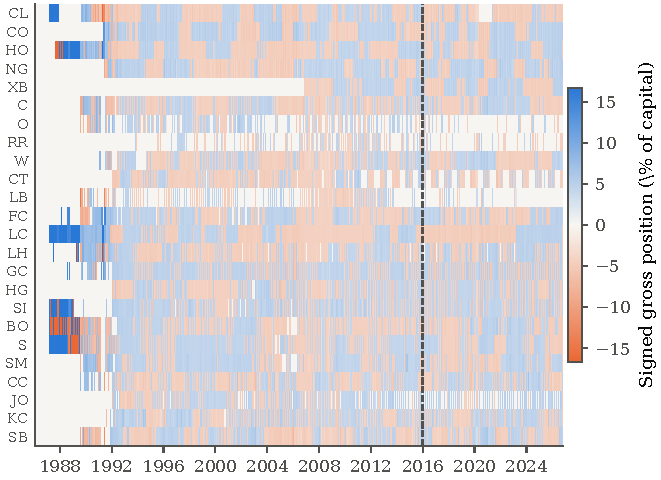
\includegraphics[width=\linewidth]{figures/d_positions.pdf}
{\scriptsize\color{slate}Month-end book: blue = long near, orange = short.}
\end{column}
\begin{column}{0.47\textwidth}
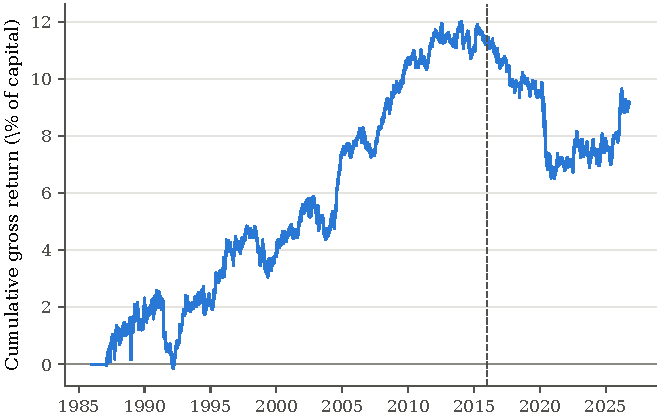
\includegraphics[width=\linewidth]{figures/d_gross_pnl.pdf}
{\scriptsize\color{slate}Gross P\&L, \$10m capital; dashed line = 2016.}
\vspace{0.5ex}
\footnotesize
\begin{itemize}
  \item Book rotates across all 24 roots; no persistent directional tilt
  \item Gross exposure $\approx100\%$ of capital; turnover $\approx22\times$/yr
  \item Gross $+0.22\%$/yr full, $-0.21\%$/yr test
\end{itemize}
\end{column}
\end{columns}
\end{frame}

% =====================================================================

\section{E: Nelson--Siegel dynamics}

\begin{frame}{E \textperiodcentered\ Nelson--Siegel curve dynamics}
\begin{center}
\begin{minipage}{0.82\linewidth}
\begin{block}{Reserved for teammate}
\footnotesize
\begin{itemize}
  \item Paper: \textcite{bianchi2023exploiting}
  \item Cover: the paper's idea, its method, our replication or alternative,
        results and robustness
  \item This section is intentionally blank in the draft
\end{itemize}
\vspace{0.5ex}
{\scriptsize\color{slate}
$\square$~Paper setup \quad
$\square$~Method \quad
$\square$~Replication \quad
$\square$~Results \quad
$\square$~Robustness}
\end{block}
\end{minipage}
\end{center}
\end{frame}

% =====================================================================
\section{Portfolio}

\begin{frame}{Putting the alphas together}
\begin{columns}[T, onlytextwidth]
\begin{column}{0.55\textwidth}
\footnotesize
\begin{itemize}
  \item Candidate inputs: \key{A flip}, \key{B flip}, C variants, D (weak),
        E (if tradable)
  \item Combination model: equal-weight, inverse-vol or shrinkage; correlation
        and turnover constraints
  \item Same v2 engine, same all-in costs, same train/test split
  \item Key question: does diversification across weak signals survive costs?
  \item Required output: combined net Sharpe, turnover, drawdown and the
        correlation matrix
\end{itemize}
\end{column}
\begin{column}{0.42\textwidth}
\figph[4.6cm]{Placeholder: combined NAV, net Sharpe and
correlation matrix.\\[2pt]
This is the remaining step, not a finished result.}
\end{column}
\end{columns}
\takeaway{Individual signals are weak. The portfolio is the only place where
their information could still add up.}
\end{frame}

% =====================================================================
\section{Conclusion}

\begin{frame}{What we learned}
\centering
{\scriptsize
\setlength{\tabcolsep}{4pt}
\begin{tabular}{@{}L{3.0cm} r r r L{2.2cm}@{}}
\toprule
Idea & Gross (\%/yr) & All-in net (\%/yr) & Gross Sharpe & Verdict \\
\midrule
A spread convergence & $+0.63$ & --- & $0.63$ & candidate (gross) \\
B relative value & $+0.50$ & --- & $1.06$ & candidate (gross) \\
C mean reversion & $+0.61$ & --- & $0.38$ & weak gross \\
D curve momentum & $+0.22$ & $-1.42$ & $0.25$ & weak / unstable \\
E Nelson--Siegel & --- & --- & --- & teammate \\
\bottomrule
\end{tabular}
\par}
\vspace{1ex}
\begin{columns}[T, onlytextwidth]
\begin{column}{0.48\textwidth}
\footnotesize
\begin{itemize}
  \item A/B convergence carry gross information; costs decide whether they
        survive the portfolio
  \item C/D contain some gross signal, but it is weak and unstable
  \item Contract-level alignment is the foundation; generic slot returns would
        be wrong
\end{itemize}
\end{column}
\begin{column}{0.48\textwidth}
\footnotesize
\begin{itemize}
  \item A/B are \key{portfolio candidates}, not standalone strategies; the
        test evidence is suggestive
  \item Next: E, portfolio combination, H holding-period scan
  \item No single idea is a standalone strategy, but the pipeline is reusable
\end{itemize}
\end{column}
\end{columns}
\end{frame}

% =====================================================================
\begin{frame}[standout]
  Thank you
  \vspace{1.5ex}

  {\normalsize Questions welcome}
  \vspace{1ex}

  {\small Jiaheng Han \& Tian Tian}
\end{frame}

% =====================================================================
\appendix

\begin{frame}{Backup: data QA}
\footnotesize
\begin{itemize}
  \item 0 duplicate contract-date rows
  \item 0 rank-order violations
  \item 0 partial rolls; 0 full-day queue violations
  \item CL 2020-04-20 settlement of $-37.63$ retained
  \item 175 tests pass; notebooks 00/01 and 10--14 run top-to-bottom
  \item All panels can be rebuilt from the raw Bloomberg CSV
\end{itemize}
\end{frame}

\begin{frame}{Backup: cost model and definitions}
\begin{columns}[T, onlytextwidth]
\begin{column}{0.48\textwidth}
\footnotesize
\begin{itemize}
  \item \key{Half-spread}: per-contract quote, paid on each leg
  \item \key{Fee}: exchange fee per contract
  \item \key{Impact}: square-root of order size / ADV
  \item All-in net = gross $-$ half-spread $-$ fee $-$ impact
  \item v1's flat 5 bps/leg is historical and is not mixed with v2
\end{itemize}
\end{column}
\begin{column}{0.48\textwidth}
\footnotesize
\begin{itemize}
  \item \key{Eligibility}: no delivery month; exit at least 5 trading days
        before; days to last trading $>D$
  \item \key{Main pair}: two nearest eligible contracts
  \item \key{Carry}: annualized near--far price difference
  \item \key{D}: research buffer; $D=10$ main, $D=5/20$ robustness
  \item \key{Test}: 2016--2026, read once and never used for tuning
\end{itemize}
\end{column}
\end{columns}
\end{frame}

\begin{frame}{Backup: A flip --- per-root 5-day IC}
\centering
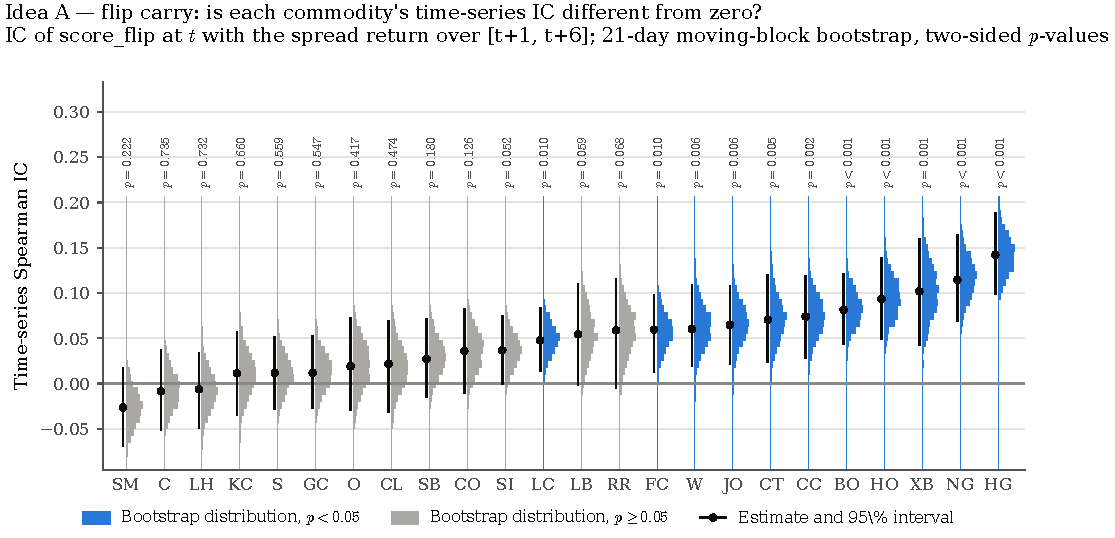
\includegraphics[width=0.86\linewidth]{figures/a_flip_ic_bootstrap.pdf}
\par\vspace{0.5ex}
{\scriptsize\color{slate}Full sample 1986--2026; 21-day block bootstrap, 2,000 draws.
Blue = $p<0.05$. 11/24 roots significant; in the test slice, 8/24 are
significant and only 1/24 has a positive 95\% CI.}
\end{frame}

\begin{frame}[allowframebreaks]{References}
\printbibliography[heading=none]
\end{frame}

\end{document}
